%%%%%%%%%%%%%%%%%%%%%%%%%%%%%%%%%%%%%%%%%%%%%%%%%%%%%%%%
% IE643 course poster, A1 portrait. Layout, colours and section order follow the course template
% (a0poster class by Kettl and Weiser, CC BY-NC-SA 3.0; design: Timothy Kodikara).
% Figures: make_figures.py (from the repo's code and logged results).
%%%%%%%%%%%%%%%%%%%%%%%%%%%%%%%%%%%%%%%%%%%%%%%%%%%%%%%%
\documentclass[a1,portrait]{a0poster}
%%
\usepackage[top=3.5cm, bottom=0.3cm, left=3.5cm, right=2cm]{geometry}
\usepackage[compact]{titlesec}
\usepackage{multicol}
\columnsep=70pt
\columnseprule=10pt
\usepackage[svgnames]{xcolor}
\usepackage{palatino}
\usepackage{xkeyval}
\usepackage{graphicx}
\setlength{\abovecaptionskip}{5pt plus 5pt minus 3pt}
\graphicspath{{figures/}}
\usepackage{booktabs}
\usepackage[font=small,labelfont=bf]{caption}
\usepackage{amsfonts, amsmath, amsthm, amssymb}
\usepackage{csquotes}
\usepackage{wrapfig}
\usepackage{multirow}
\usepackage{makecell}
\def\columnseprulecolor{\color{NavyBlue}}%
\usepackage{framed}
\colorlet{frameborder}{NavyBlue}
\begin{document}
\begin{minipage}[c]{\linewidth}
\vspace{0.1cm}
\noindent\makebox[\textwidth][c]{
\begin{minipage}[c]{0.14\linewidth}
\vspace{0pt}\raggedright
\hspace{1cm}

\includegraphics[scale=1.3,width=\linewidth]{figures/logo.png}
\end{minipage}
\hfill
\begin{minipage}[c]{0.75\textwidth}
\centering
\Huge \color{Green} \textbf{IE643 Course Project}\\[0.4cm]
\Huge \color{NavyBlue} \textbf{Constraint Driven Multimodal Diffusion\\ using Text, Sketch and Reference Image}\\[0.4cm]
\Large \color{NavyBlue} \textbf{One Sheep Army}\\[0.4cm]
\large \color{Black} \textbf{Team Member Name 1 $^{1}$ (Roll Number), Team Member Name 2 $^{2}$} (Roll Number)\\[0.2cm]
\small \text{XXXX@iitb.ac.in$^{1}$, XXXXX@iitb.ac.in$^{2}$}\\
\end{minipage}
\begin{minipage}[c]{0.145\textwidth}
\vspace{0pt}\raggedleft

\includegraphics[scale=1.3,width=\linewidth]{figures/IE643-Logo.pdf}
\hspace{1cm}
\end{minipage}}
\\[0.1cm]%
\color{NavyBlue}\setlength\FrameRule{18pt}
\begin{framed}
\vspace{0.4cm}
\begin{multicols}{2}
%----------------------------------------------------------------------------------------
\color{Black}
\section*{Abstract}
One object is generated from a text caption, a sketch and a reference image, which may disagree. We fix who governs what:
sketch $\rightarrow$ shape, text $\rightarrow$ identity, reference $\rightarrow$ colour and material. We submit a frozen SDXL driven by a
\textbf{neutral caption plus a higher IP-Adapter scale}. \textbf{This is a rule applied outside the model; SDXL does not learn the roles.}

%----------------------------------------------------------------------------------------
\section*{Introduction}
\begin{itemize}
	\item Inputs can conflict: caption says ``purple'', reference is silver.
	\item Rule: the reference wins colour, even against the caption.
\end{itemize}
\begin{center}
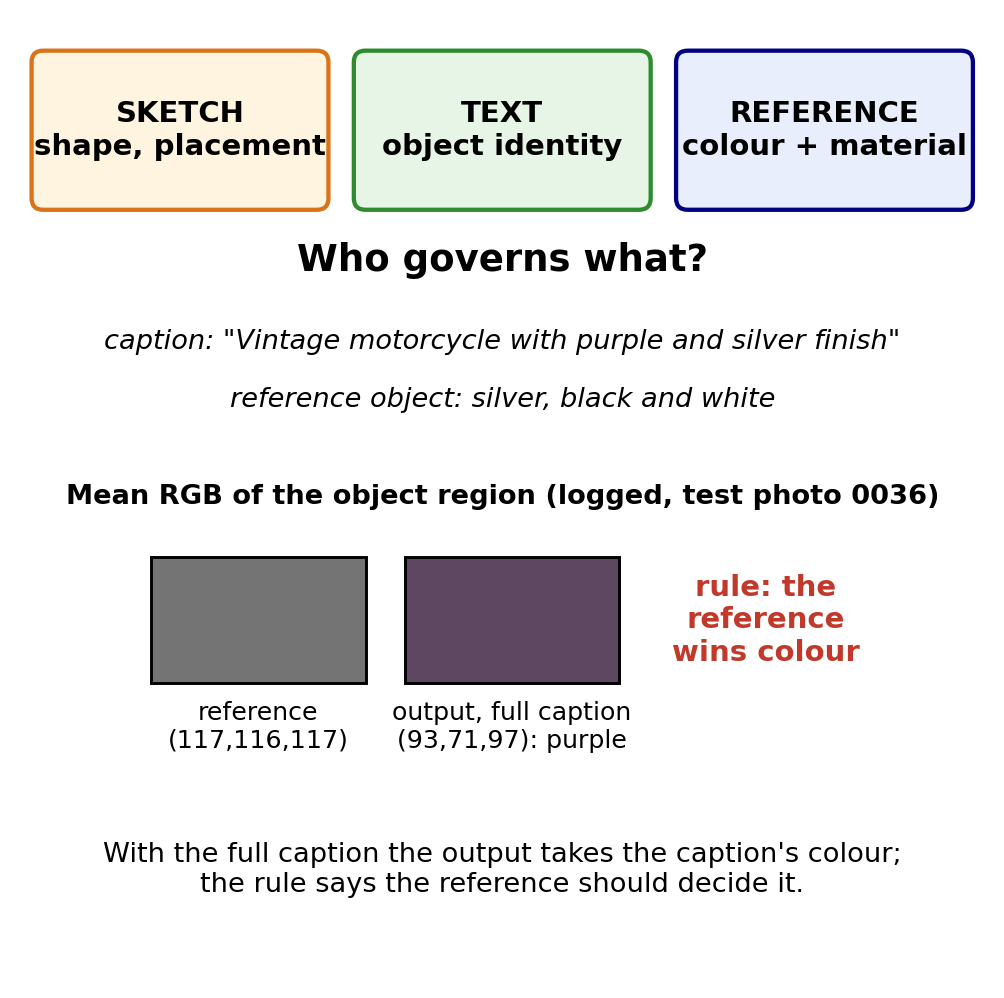
\includegraphics[width=0.3\linewidth]{figures/Intro.png}
\captionof{figure}{\color{Blue}Logged mean object colour of an output made with the full caption, versus its reference.}
\label{Intro}
\end{center}
We outline our major \textbf{contributions} below:
\vspace{-\baselineskip}\\
\begin{itemize}
	\item A per-attribute governing rule and a labelled conflict test set.
	\item Neutral caption + IP scale on frozen SDXL, ControlNet and IP-Adapter.
	\item Role-compliance evaluation, with the failed learned variants reported.
\end{itemize}

%----------------------------------------------------------------------------------------
\color{Black}
\section*{Workflow}
Figure \ref{workflow} illustrates the workflow, from photos to per-conflict evaluation.
\begin{center}
	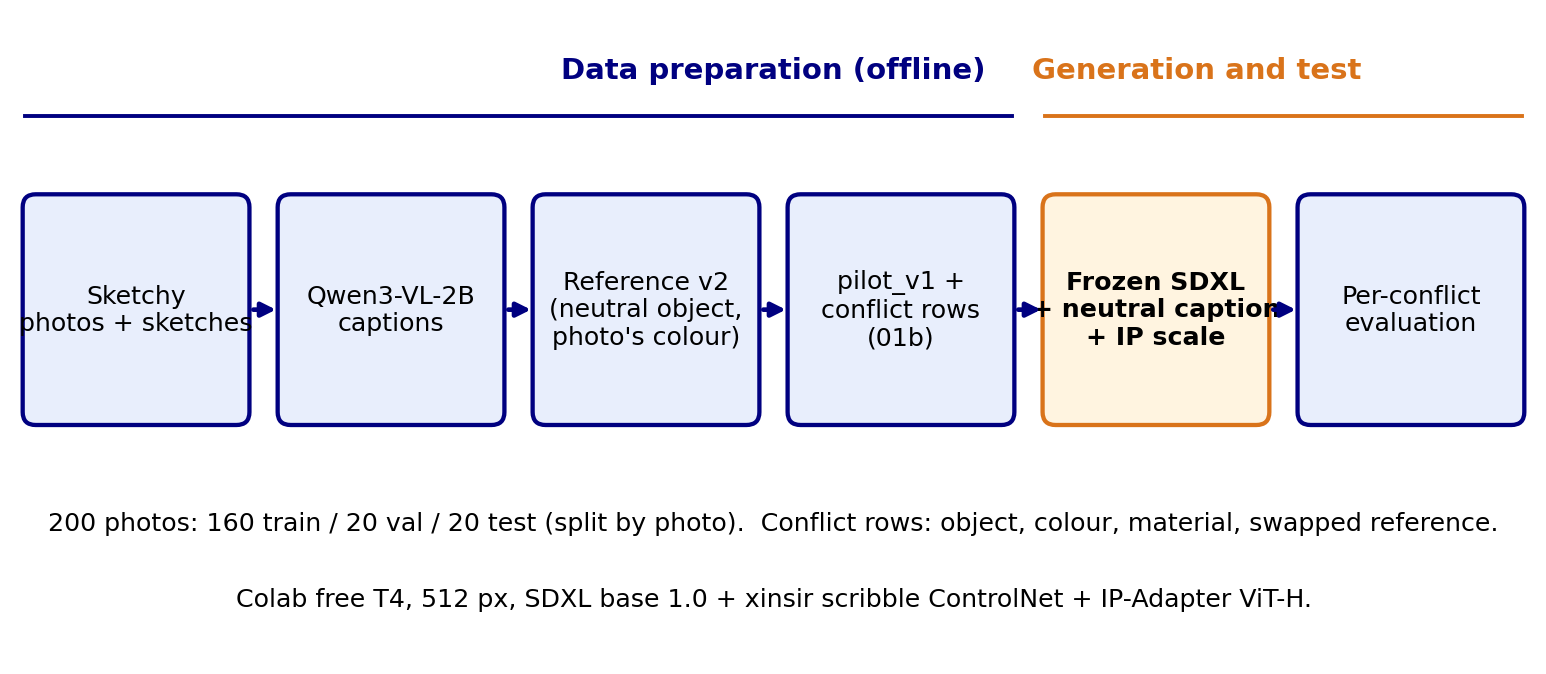
\includegraphics[width=0.65\linewidth]{figures/Workflow.png}
	\captionof{figure}{\color{Blue} Overall Workflow}
	\label{workflow}
\end{center}

%----------------------------------------------------------------------------------------
\section*{Methodology}
Figure \ref{Arch} illustrates the architecture. The rule (red) acts on the inputs of a frozen SDXL.
\begin{itemize}
	\item \textbf{Neutral caption:} colour words $\rightarrow$ ``colored'', material words $\rightarrow$ ``solid'', in the UNet text, pooled embedding and ControlNet text.
	\item \textbf{IP scale:} 0.5 $\rightarrow$ 1.0, so the reference decides colour and material.
\end{itemize}
\begin{center}
	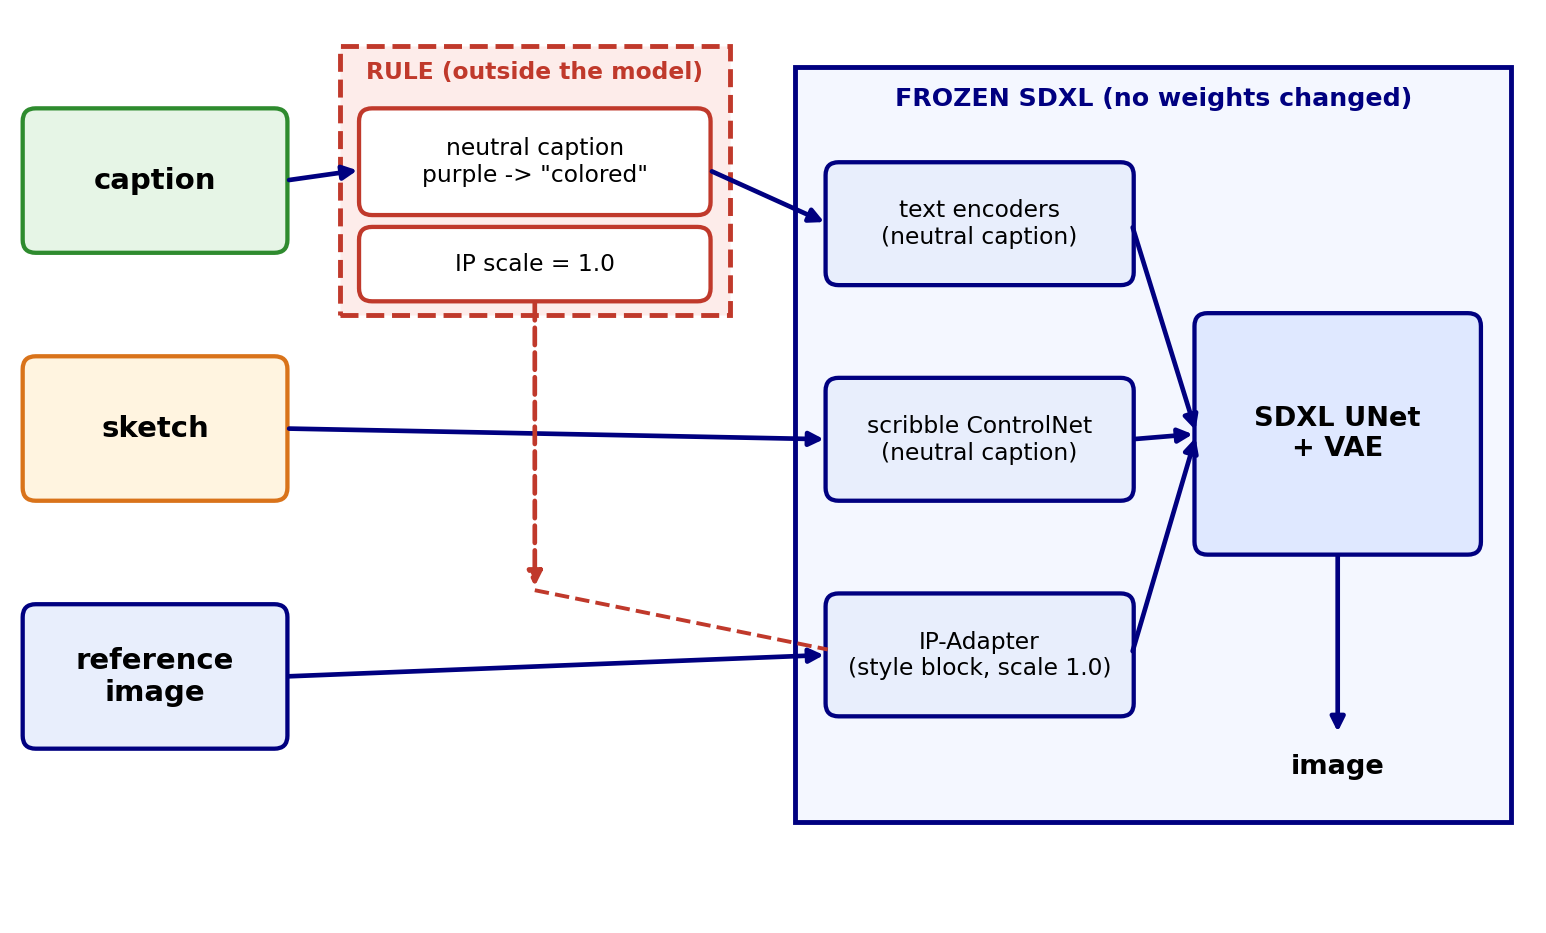
\includegraphics[width=0.58\linewidth]{figures/Deep-Neural-Network-Model.png}
	\captionof{figure}{\color{Blue} Overall Architecture}
	\label{Arch}
\end{center}

%----------------------------------------------------------------------------------------
\color{Black}
\section*{Dataset Details}
Sketchy database; 200 captioned photos (Qwen3-VL-2B), split 160/20/20 by photo, each with a sketch, a neutral-object reference carrying the
photo's colour and material, and labelled object, colour, material and swapped-reference conflict rows. Evaluated on 12 test photos, 10 rows per conflict type.

%----------------------------------------------------------------------------------------
\color{Black}
\section*{Novelty Assessment}
Learned ways to make the model resolve conflicts itself, all tried and not adopted:
\begin{itemize}
	\item \textbf{Router and governance network:} flags conflicts, but images did not change.
	\item \textbf{Fusion LoRA:} object conflicts 8/8, but edge IoU fell 0.369 $\rightarrow$ 0.230.
	\item \textbf{Role gates, colour adapter:} gates barely moved; palettes ignored.
\end{itemize}
Leak test: the ControlNet saw the full caption, so ``purple'' leaked through. The neutral caption closes that path.

%----------------------------------------------------------------------------------------
\color{Black}
\section*{Results}
Share of rows where the governing input won (12 photos, 10 rows per type; indicative).
\begin{center}
	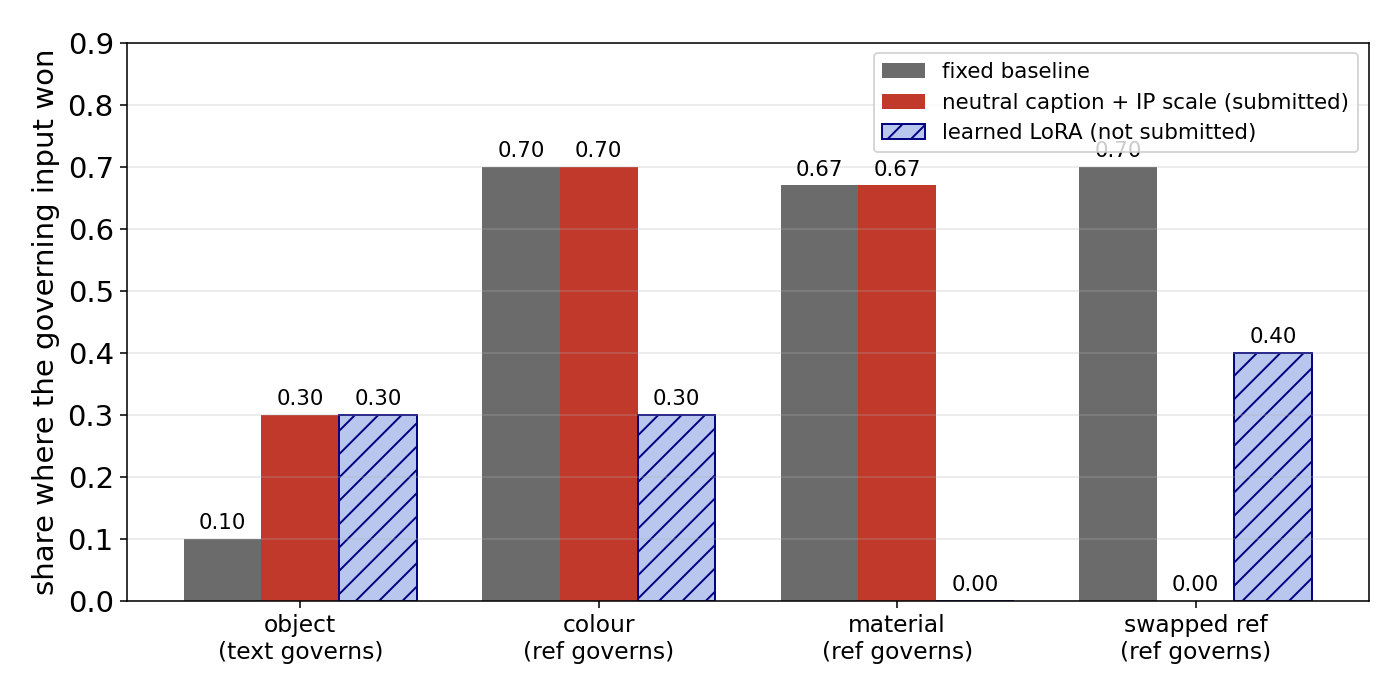
\includegraphics[width=0.5\linewidth]{figures/results_compliance.png}
	\captionof{figure}{\color{Blue} Role compliance per conflict type.}
\end{center}

\begin{center}
	\scalebox{0.72}{
		\begin{tabular}{|l|c|c|c|c|}
			\hline
			Methods & edge IoU & edge IoU (conflict) & DINO to target & CLIP-T \\
			\hline
			Fixed baseline & 0.213 & 0.221 & \textbf{0.359} & \textbf{0.263} \\
			\textbf{Ours (neutral caption + IP scale)} & \textbf{0.376} & \textbf{0.375} & 0.300 & 0.246 \\
			Role LoRA (not submitted) & 0.753 & 0.753 & 0.057 & 0.220 \\
			\hline
		\end{tabular}}\\
\captionof{table}{\color{Blue} Sketch and fidelity metrics.}\label{table}
	\vspace{-0.25in}
\end{center}
\vspace{0.25in}
Gains in object identity and sketch fidelity. No gain in colour and material (0.70, 0.67), and a loss on swapped references (0.00 vs 0.70).

%----------------------------------------------------------------------------------------
\color{Black}
\section*{Conclusion}
\begin{itemize}
	\item Submitted: neutral caption plus IP scale, \textbf{a rule applied outside the model}.
	\item Better sketch fidelity and object identity; unchanged colour and material; worse on swapped references.
	\item Having the model itself resolve conflicts remains open.
\end{itemize}
%----------------------------------------------------------------------------------------
\begin{thebibliography}{3}

\bibitem {SDXL}
Podell, D., et al.: SDXL: Improving latent diffusion models for high-resolution image synthesis. ICLR (2024)

\bibitem {IPA}
Ye, H., et al.: IP-Adapter: Text compatible image prompt adapter for text-to-image diffusion models. arXiv:2308.06721 (2023)

\bibitem {CN}
Zhang, L., Rao, A., Agrawala, M.: Adding conditional control to text-to-image diffusion models. ICCV (2023)

\end{thebibliography}
%----------------------------------------------------------------------------------------
\section*{Acknowledgments}
\small \textnormal{We thank the IE643 teaching staff.}

\section*{Github Link and Demo Video Link}
\vspace{-0.5cm}

\begin{center}
		\begin{minipage}{0.4\linewidth}
			\centering
			\textbf{Github Repository}\\[1ex]
			
\includegraphics[width=0.5\linewidth]{Repo_QR.png}
		\end{minipage}\hfill
		\begin{minipage}{0.4\linewidth}
			\centering
			\textbf{Demo Video Link}\\[1ex]
			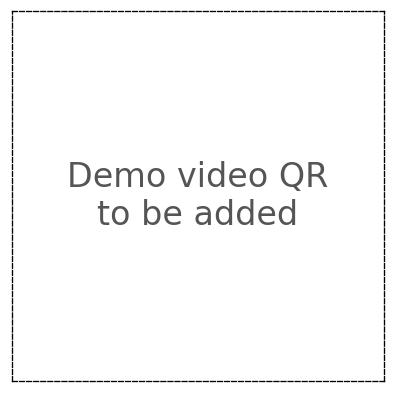
\includegraphics[width=0.5\linewidth]{Demo_QR_placeholder.png}
		\end{minipage}
\end{center}


\end{multicols}
\vspace{0.4cm}
\end{framed}
\end{minipage}
\end{document}
